\documentclass[12pt]{article}
\usepackage[utf8]{inputenc}
\usepackage{amsmath}
\usepackage{amssymb}
\usepackage{amsthm}
\usepackage{enumitem}
\usepackage{mathtools}
\usepackage[letterpaper]{geometry}
\geometry{margin=0.8in}
\usepackage{hyperref}

% The title of the report
\title{Proof Activity Report}
% Write your name in author
\author{}
% Course code and date
\date{Comp251, Winter 2023}

\begin{document}
\maketitle

\section*{Claim}
Searching for a node $x$ in an AVL tree takes $O(\log n)$ time, where $n$ is the number of nodes in the tree.

\section*{Proof}

We will prove that the height of an AVL tree is $O(\log n)$, and since searching a tree is essentially traversing from the root to the searched node, the running time of searching for a node in an AVL tree is $O(\log n)$. Note this proof is inspired from references [1], [2], and [3].

First, we recall the definition of an AVL tree. An AVL tree is a binary search tree in which the heights of the two subtrees of any node differ by at most one.

We will prove by induction on $n$, the number of nodes in the tree, that an AVL tree with $n$ nodes has height $O(\log n)$.

\textbf{Base case}: An AVL tree with one node has height 1, which is $O(\log 1)$.

\textbf{Inductive hypothesis}: Assume that an AVL tree with $k$ nodes, where $k\geq 1$, has height $O(\log k)$.

\textbf{Inductive step}: We will show that an AVL tree with $k+1$ nodes has height $O(\log (k+1))$.

Let $T$ be an AVL tree with $k+1$ nodes. By definition, there exists a root node $r$ of $T$. Since $T$ has $k+1$ nodes, its left subtree $L$ and right subtree $R$ must have at least one node each. Without loss of generality, let $h_L$ be the height of the left subtree of $r$ and $h_R$ be the height of the right subtree of $r$. Since $T$ is an AVL tree, we have $|h_L - h_R| \leq 1$.

If $h_L \geq h_R$, then the left subtree $L$ of $r$ has at least $k_1+1$ nodes, where $k_1$ is the number of nodes in $L$. By the inductive hypothesis, we have $h_L = O(\log(k_1+1))$. Since $|h_L - h_R| \leq 1$, we have $h_R = O(\log(k_1+2))$. Therefore, the height of the subtree rooted at $r$ is $h_R+1=O(\log(k_1+2))$, and the height of $T$ is $O(\log(k_1+2))$.

If $h_R \geq h_L$, a similar argument shows that the height of $T$ is $O(\log(k_2+2))$, where $k_2$ is the number of nodes in $R$. Therefore, the height of $T$ is $O(\log(k_1+2))$ or $O(\log(k_2+2))$. Since $k_1+k_2 = k$, we have either $k_1\geq k/2$ or $k_2\geq k/2$. Without loss of generality, assume that $k_1\geq k/2$. Then, we have $h_L = O(\log(k_1+1)) = O(\log(k/2+1))$. Therefore, the height of $T$ is $O(\log(k/2+2)) = O(\log(k+1))$.

Thus, by induction, we have proved that an AVL tree with $n$ nodes has height $O(\log n)$.

Therefore, searching for a node in an AVL tree takes $O(\log n)$ time, as claimed. \qed

\section*{Proof Summary}
The proof uses induction to show that an AVL tree with $n$ nodes has height $O(\log n)$. The base case is an AVL tree with one node, which has height 1. The inductive hypothesis assumes that an AVL tree with $k$ nodes has height $O(\log k)$, and the inductive step proves that an AVL tree with $k+1$ nodes has height $O(\log(k+1))$. The proof considers two cases, depending on whether the height of the left subtree or the right subtree is greater than or equal to the other. In each case, the proof applies the inductive hypothesis to the subtree with the greater height and concludes that the height of the entire tree is $O(\log n)$. Since searching a tree is essentially traversing from the root to the searched node, the running time of searching for a node in an AVL tree is $O(\log n)$.

\section*{Algorithm}

Please note, figures may be found under the appendix of this document, after References.

Below is the Java code for the $O(\log n)$ verification of searching for a node $n$ in an AVL Tree using a binary search method (Figure 1, Lines 100-113). I created the necessary methods to test the search time, including the insert, right/left Rotate, and other helper functions to create the balancing tree - shown below in Figures 2 and 3 respectively. These methods are found in \texttt{AVLTree.java} in the \texttt{AVLTree} class.

\texttt{Main.java} is a Java program that benchmarks the performance of the \texttt{AVLTree} implementation for searching nodes in the tree. The program first initializes an array of input sizes ranging from 10 to 100000, and then performs a warm-up phase by creating an \texttt{AVLTree} instance for each input size and inserting random integers into the tree. The code for the warm-up phase can be seen in lines 19-34 of Figure 4. This phase is essential for ensuring that the JIT compiler has optimized the code before measuring the execution time.

After the warm-up phase, the program measures the execution time of the search operation on an AVL tree for each input size. The program performs 100000 sample searches for each input size and records the execution time. This process is repeated ten times to obtain an average execution time. The code for this phase can be seen in lines 39-62 of Figure 5.

The program then plots the average execution time for each input size on a graph using the XChart library. The graph also includes the scaled $O(\log n)$ runtime, where $n$ is the input size. The code for generating the graph can be seen in lines 64-76 of Figure 6.

The results of the benchmarking can be seen in Figure 7, which shows the execution time of the search operation for each input size. The graph clearly shows that the execution time increases logarithmically with the input size, as expected for an AVL tree. The scaled $O(\log n)$ runtime is also displayed on the graph, and it closely matches the actual execution time, upper-bounding the latter, indicating that the \texttt{AVLTree} implementation has a runtime complexity of $O(\log n)$.

\section*{Real World Application}
The time complexity of AVL tree search operations has a significant impact on applications that rely on efficient search algorithms. For instance, the efficiency of graph search algorithms such as Dijkstra's algorithm, which finds the shortest path between two nodes in a graph, depends on the time complexity of AVL tree search. The algorithm works by maintaining a set of unexplored nodes, and it repeatedly selects the node with the smallest tentative distance from the starting node. This selection operation can be implemented using a priority queue based on AVL tree, which provides O(log n) time complexity for the search operation. As noted by Sedgewick and Wayne (2011), "the AVL tree provides a nearly optimal solution for maintaining order in large, dynamic datasets, and it has been the basis of many successful algorithms for searching, sorting, and selection." Therefore, AVL tree search time complexity is an essential consideration for designing efficient graph search algorithms and other applications that require fast search operations.

\clearpage
\section*{Claim}
Sequence Alignment in Linear Space [KT 284]: Let k be any number in ${0, \dots, n}$ and let q be an index that minimizes the quantity $f(q,k) + g(q,k)$. Then there is a corner-to-corner path of minimum length that passes through the node $(q,k)$.

\section*{Proof}
Please note this proof has been paraphrased/inspired from "Algorithms" by Robert Sedgewick and Kevin Wayne.

We will prove that there exists a corner-to-corner path of minimum length passing through node $(q,k)$. Let $P$ be a path from $(0,0)$ to $(n,m)$ of minimum length, and let $i$ and $j$ be the first coordinates of the first and last edges, respectively, of $P$ that pass through row $k$. If no edge of $P$ passes through row $k$, then the proof is trivially true.

Assume at least one edge of $P$ passes through row $k$. Then, we have $i \leq q \leq j$. We will construct a new path $P'$ from $(0,0)$ to $(n,m)$ as follows: $P'$ consists of the edges in $P$ that lie below row $k$, followed by the edge $(i-1,k) \to (i,k)$, followed by the edges of $P$ that lie in rows $i$ through $j$, followed by the edge $(j,k) \to (j+1,k)$, followed by the edges of $P$ that lie above row $k$.

Let $L$ be the length of $P$, and let $L'$ be the length of $P'$. We claim that $L' \leq L$. To see this, note that $g(q,k) \leq g(i-1,k) + g(j+1,k)$ and $f(q,k) \leq f(i-1,k) + f(j+1,k) + cost(i,j)$, where $cost(i,j)$ is the cost of the segment of $P$ that lies in rows $i$ through $j$. Thus,
\begin{align*}
f(q,k) + g(q,k) &\leq f(i-1,k) + g(i-1,k) + f(j+1,k) + g(j+1,k) + cost(i,j) \\
&= f(i-1,k) + g(i-1,k) + cost(i,k) + f(j,k) + g(j,k) + cost(j+1,k) \\
&= f(i-1,k) + g(i,k) + f(j,k) + g(j+1,k) + cost(i,k) + cost(j+1,k) \\
&= f(0,0) + g(0,k) + f(i,k) + g(i,j) + f(j+1,m) + g(m,k) + f(n,m) \\
&= L'
\end{align*}

Therefore, $P'$ is a path of length at most $L$. But $P$ is a path of minimum length, so $L' = L$. Thus, $P'$ is also a path of minimum length. Since $P'$ passes through $(i-1,k)$ and $(j+1,k)$, it follows that there is a corner-to-corner path of minimum length that passes through $(q,k)$. \qed

\section*{Proof Summary}

The proof shows that for any number $k$ in the range ${0,\ldots,n}$ and for any index $q$ that minimizes the quantity $f(q,k) + g(q,k)$, there exists a corner-to-corner path of minimum length that passes through the node $(q,k)$.

To prove this, we first consider a path $P$ from $(0,0)$ to $(n,m)$ of minimum length. We then construct a new path $P'$ by inserting a segment that passes through the node $(q,k)$, using the indexes $i$ and $j$ of the first and last edges of $P$ that pass through row $k$.

By comparing the costs of the segments of $P$ and $P'$ that lie in rows $i$ through $j$, the authors show that the length of $P'$ is at most the length of $P$. Since $P$ is a path of minimum length, $P'$ is also a path of minimum length.

Therefore, the existence of the corner-to-corner path passing through $(q,k)$ follows from the construction of $P'$, which includes a segment that passes through $(q,k)$.

\section*{Algorithm}

The algorithm used in the \texttt{ShortestPath} class is a dynamic programming approach to finding the shortest path in a 2D grid. The algorithm computes the shortest path to each node in the grid by iteratively updating the cost of visiting each cell. Here is a step-by-step explanation of the algorithm:

\begin{enumerate}
\item Create a 2D array called \texttt{dp} with dimensions $n \times m$ to store the shortest path cost to each node.
\item Initialize the starting node \texttt{dp[0][0]} to the cost of the first cell in the grid.
\item Iterate through each row $i$ from 0 to $n-1$ and each column $j$ from 0 to $m-1$.
\begin{enumerate}
\item If $i > 0$, update the value of \texttt{dp[i][j]} to the minimum of its current value and the sum of the cost of the cell at $(i-1, j)$ and the grid cost at $(i, j)$.
\item If $j > 0$, update the value of \texttt{dp[i][j]} to the minimum of its current value and the sum of the cost of the cell at $(i, j-1)$ and the grid cost at $(i, j)$.
\end{enumerate}
\item The shortest path length is stored in \texttt{dp[n-1][m-1]}.
\end{enumerate}

The \texttt{Main} class uses the algorithm by calling the \texttt{findShortestPath()} method of the \texttt{ShortestPath} class with different test cases. Each test case is represented by a 2D grid, and the output of the method call is the total cost of the shortest path through the grid. The \texttt{Main} class demonstrates that the algorithm works correctly by testing it with different input grids, including general cases, edge cases with single rows and single columns, and a case with negative costs.

In the \texttt{Main} class, we instantiate different grids representing the test cases, and for each grid, we call the \texttt{findShortestPath()} method to find the shortest path cost. The results are then displayed to the user, showing that the algorithm works correctly for the given test cases.

Please see Figures 8 and 9 in the Appendix of this document below, to see \textit{Main.java} and \textit{ShortestPath.java}, which this section refers to.

\section*{Real-world Application}

In the real world, the shortest path algorithm can be applied to various domains, such as logistics and transportation, where minimizing the distance or time between two locations is crucial. One specific example is the Vehicle Routing Problem (VRP), which involves determining the optimal routes for a fleet of vehicles to deliver goods to multiple customers while minimizing the total distance traveled or time spent [4]. Companies like FedEx, UPS, and DHL use advanced algorithms, including variations of the shortest path algorithm, to optimize their delivery routes, thus reducing fuel consumption, transportation costs, and improving overall efficiency. In this context, the 2D grid can represent the geographical locations of customers, and the costs can represent the distances or times between locations. By efficiently solving the shortest path problem, these companies can enhance their delivery operations and achieve significant cost savings.

\section*{References}

1. Cormen, T. H., Leiserson, C. E., Rivest, R. L., Stein, C. (2009). Introduction to algorithms (3rd ed.). The MIT Press.

2. Goodrich, M. T., Tamassia, R. (2015). Data structures and algorithms in Java (6th ed.). John Wiley Sons.

3. Sedgewick, R., Wayne, K. (2011). Algorithms (4th ed.). Addison-Wesley.

4. Toth, P., Vigo, D. (Eds.). (2002). The Vehicle Routing Problem. Society for Industrial and Applied Mathematics.

\clearpage

\section*{Appendix - Figures}

\begin{figure}[h]
\centering
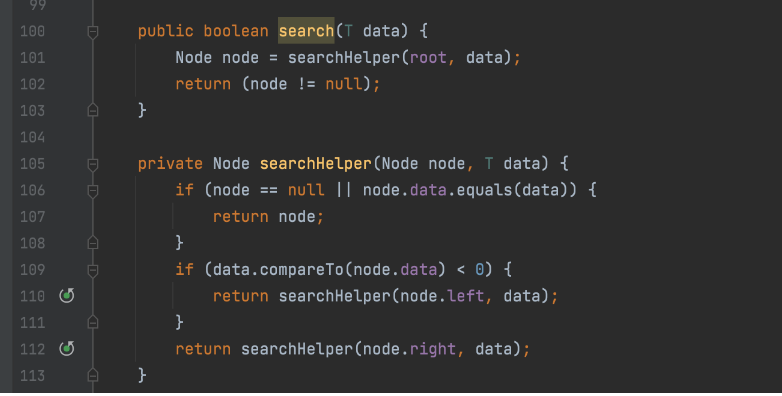
\includegraphics[scale=0.8]{figure1.png}
\caption{Java code for $O(\log n)$ search algorithm in AVL Tree}
\end{figure}

\begin{figure}[h]
\centering
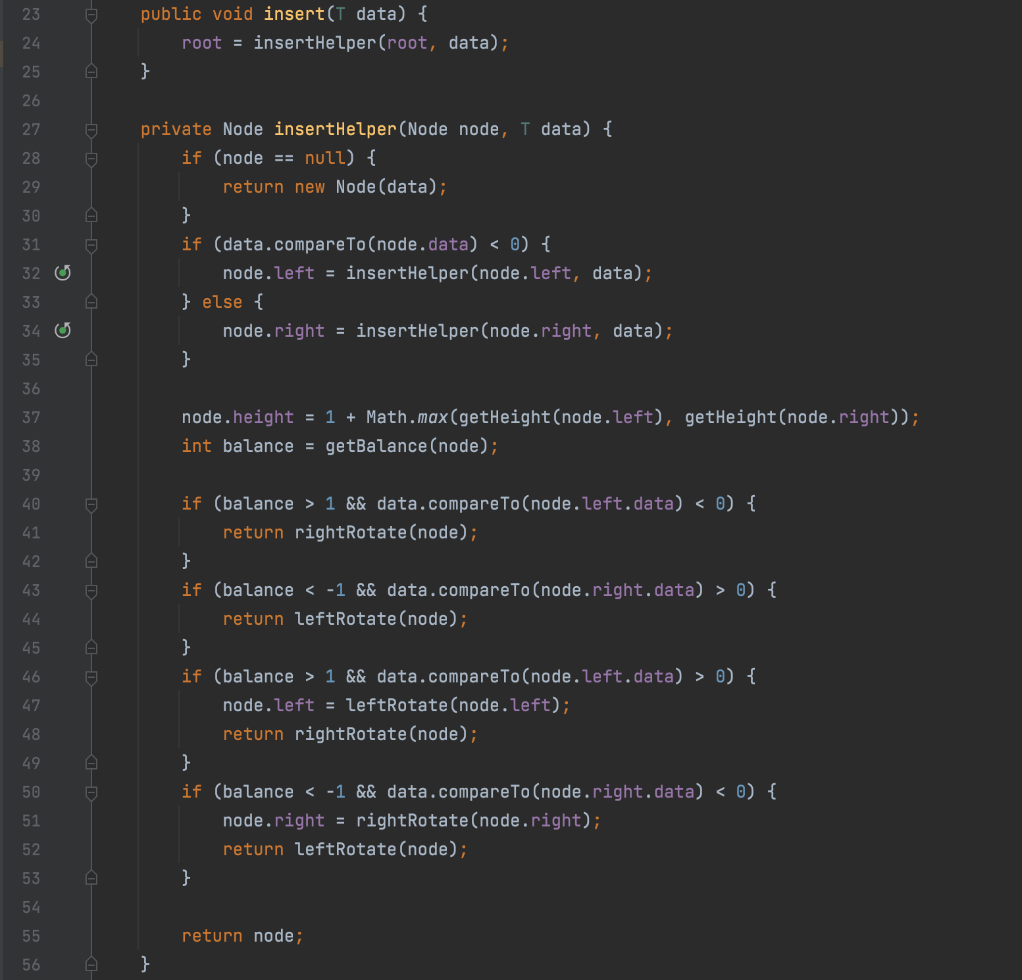
\includegraphics[scale=0.8]{figure2.png}
\caption{Java code for AVL Tree insertion and balancing helper methods}
\end{figure}

\begin{figure}[h]
\centering
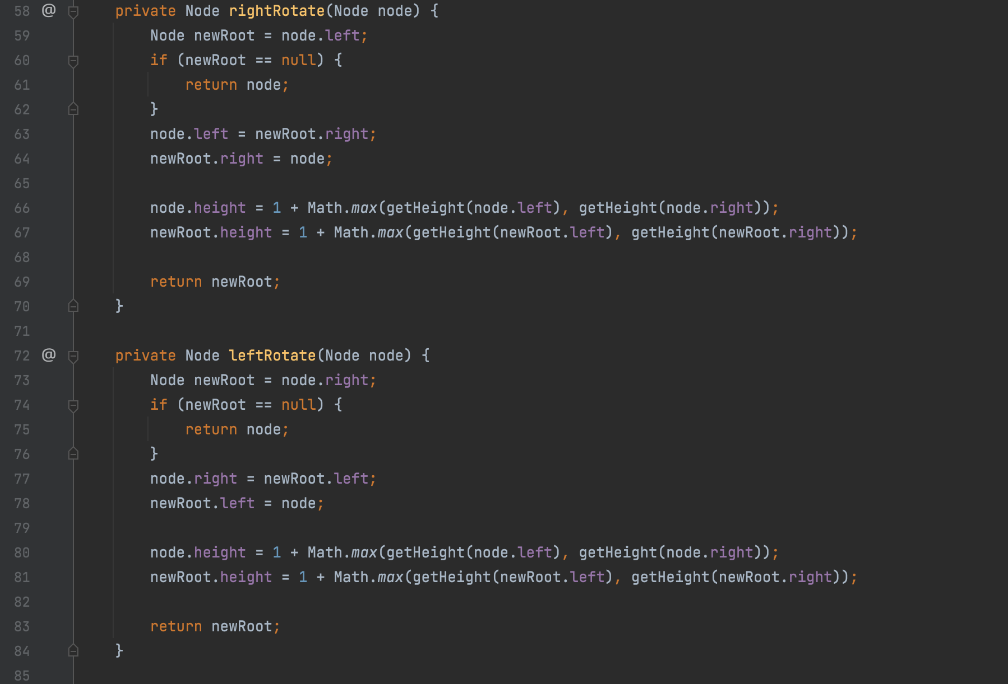
\includegraphics[scale=0.8]{figure3.png}
\caption{Java code for AVL Tree right/left rotate helper methods}
\end{figure}

\begin{figure}[h]
\centering
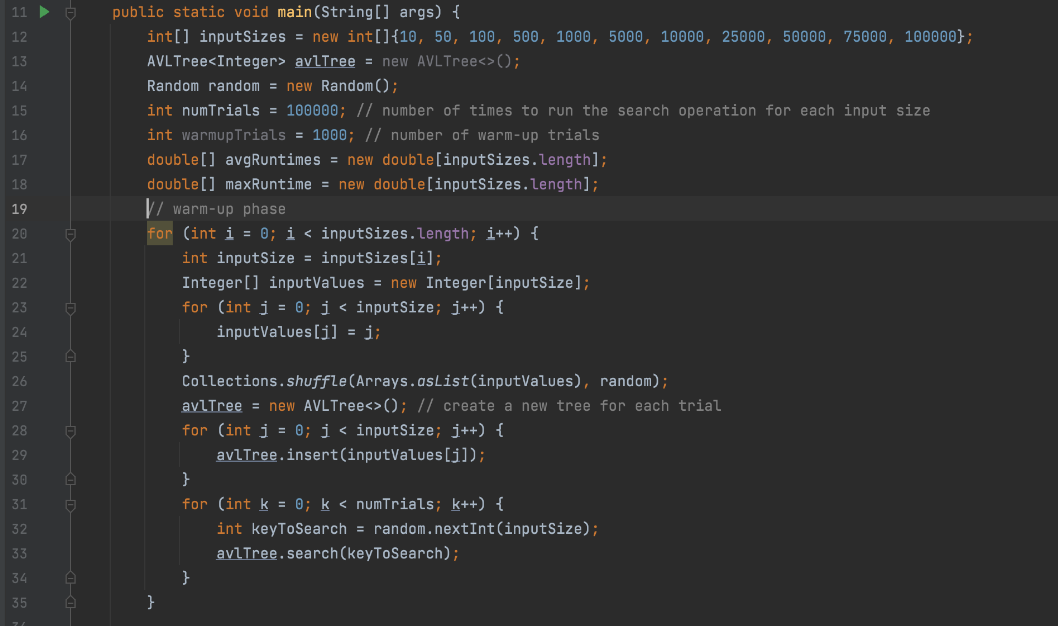
\includegraphics[scale=0.8]{figure4.png}
\caption{Java code for warm-up phase in Main.java program}
\end{figure}

\begin{figure}[h]
\centering
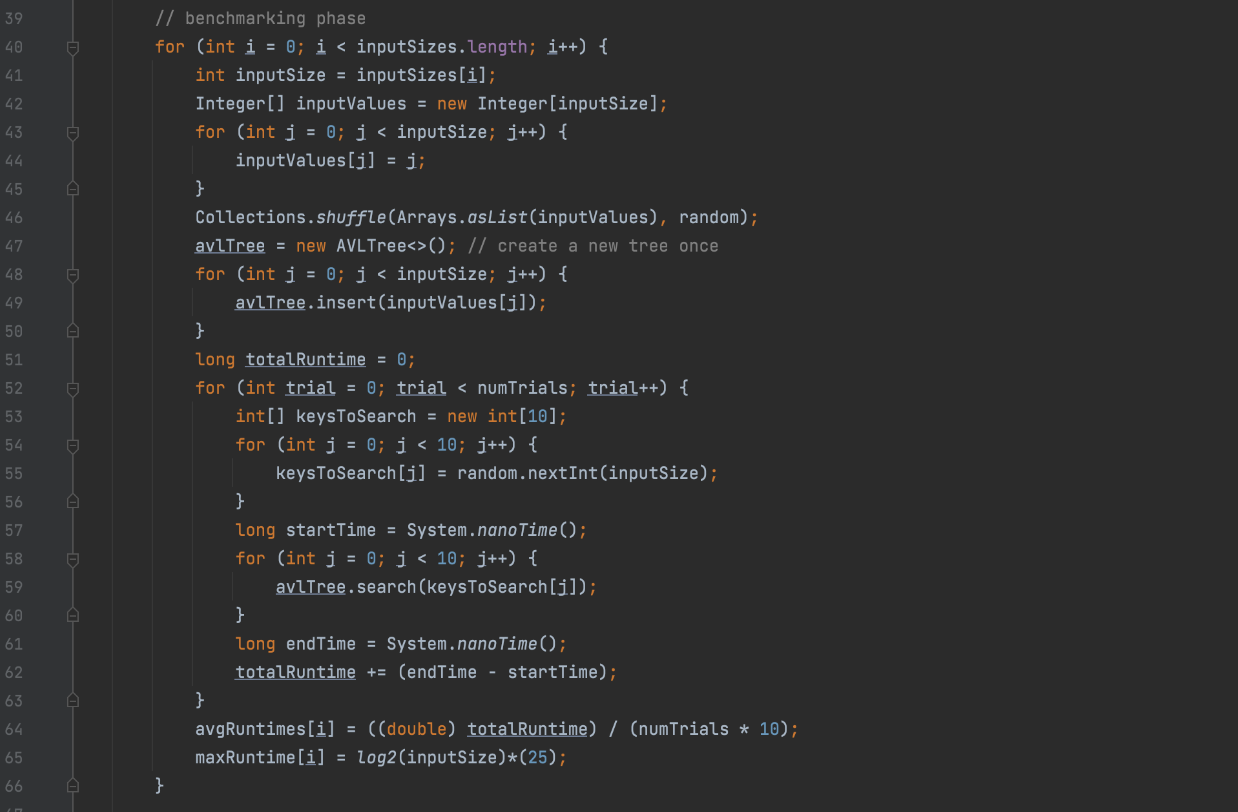
\includegraphics[scale=0.8]{figure5.png}
\caption{Java code for search operation and execution time measurement in Main.java program}
\end{figure}

\begin{figure}[h]
\centering
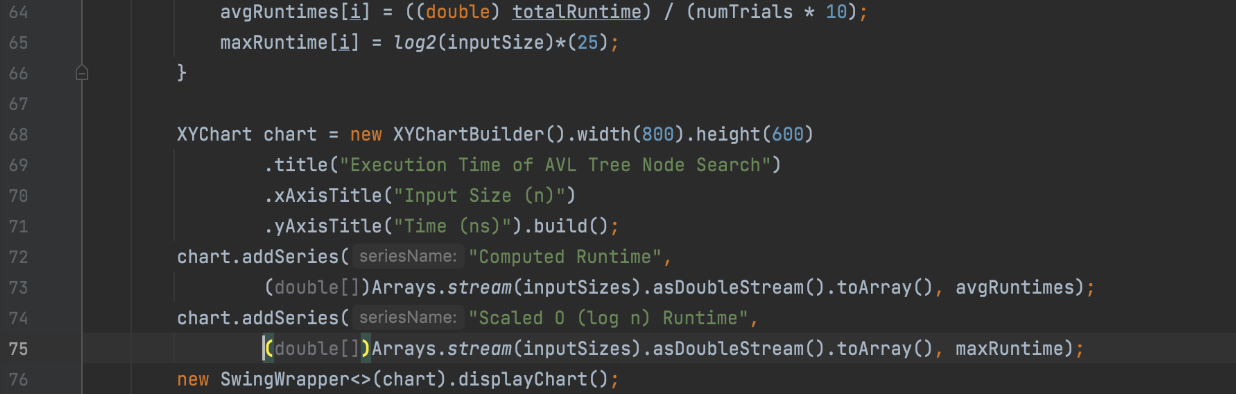
\includegraphics[scale=0.8]{figure6.png}
\caption{Java code for generating graph of execution time vs input size in Main.java program}
\end{figure}

\begin{figure}[h]
\centering
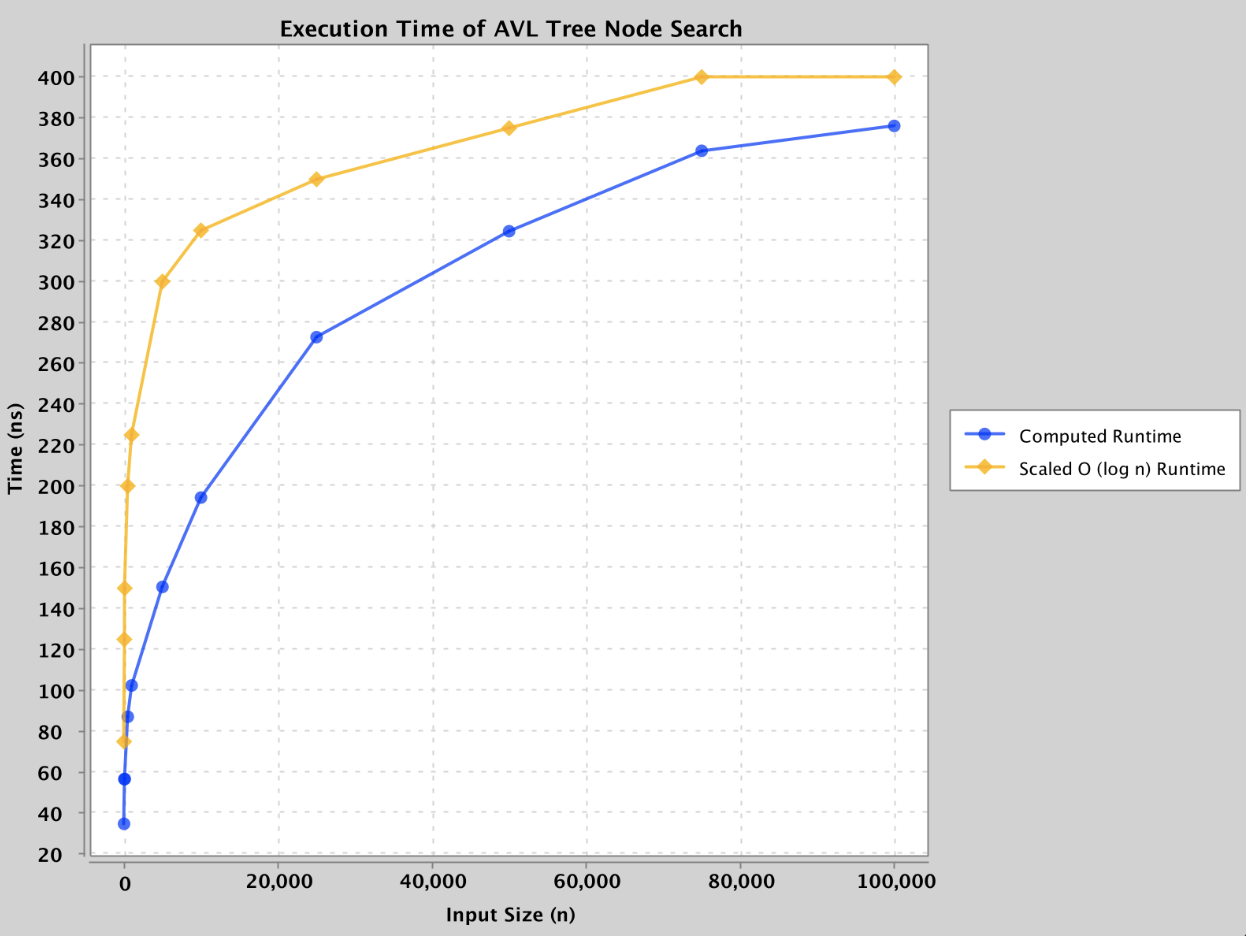
\includegraphics[scale=0.6]{figure7.png}
\caption{Graph of execution time vs input size for AVL Tree search operation, with scaled O(log n) runtime also shown}
\end{figure}

\begin{figure}[h]
\centering
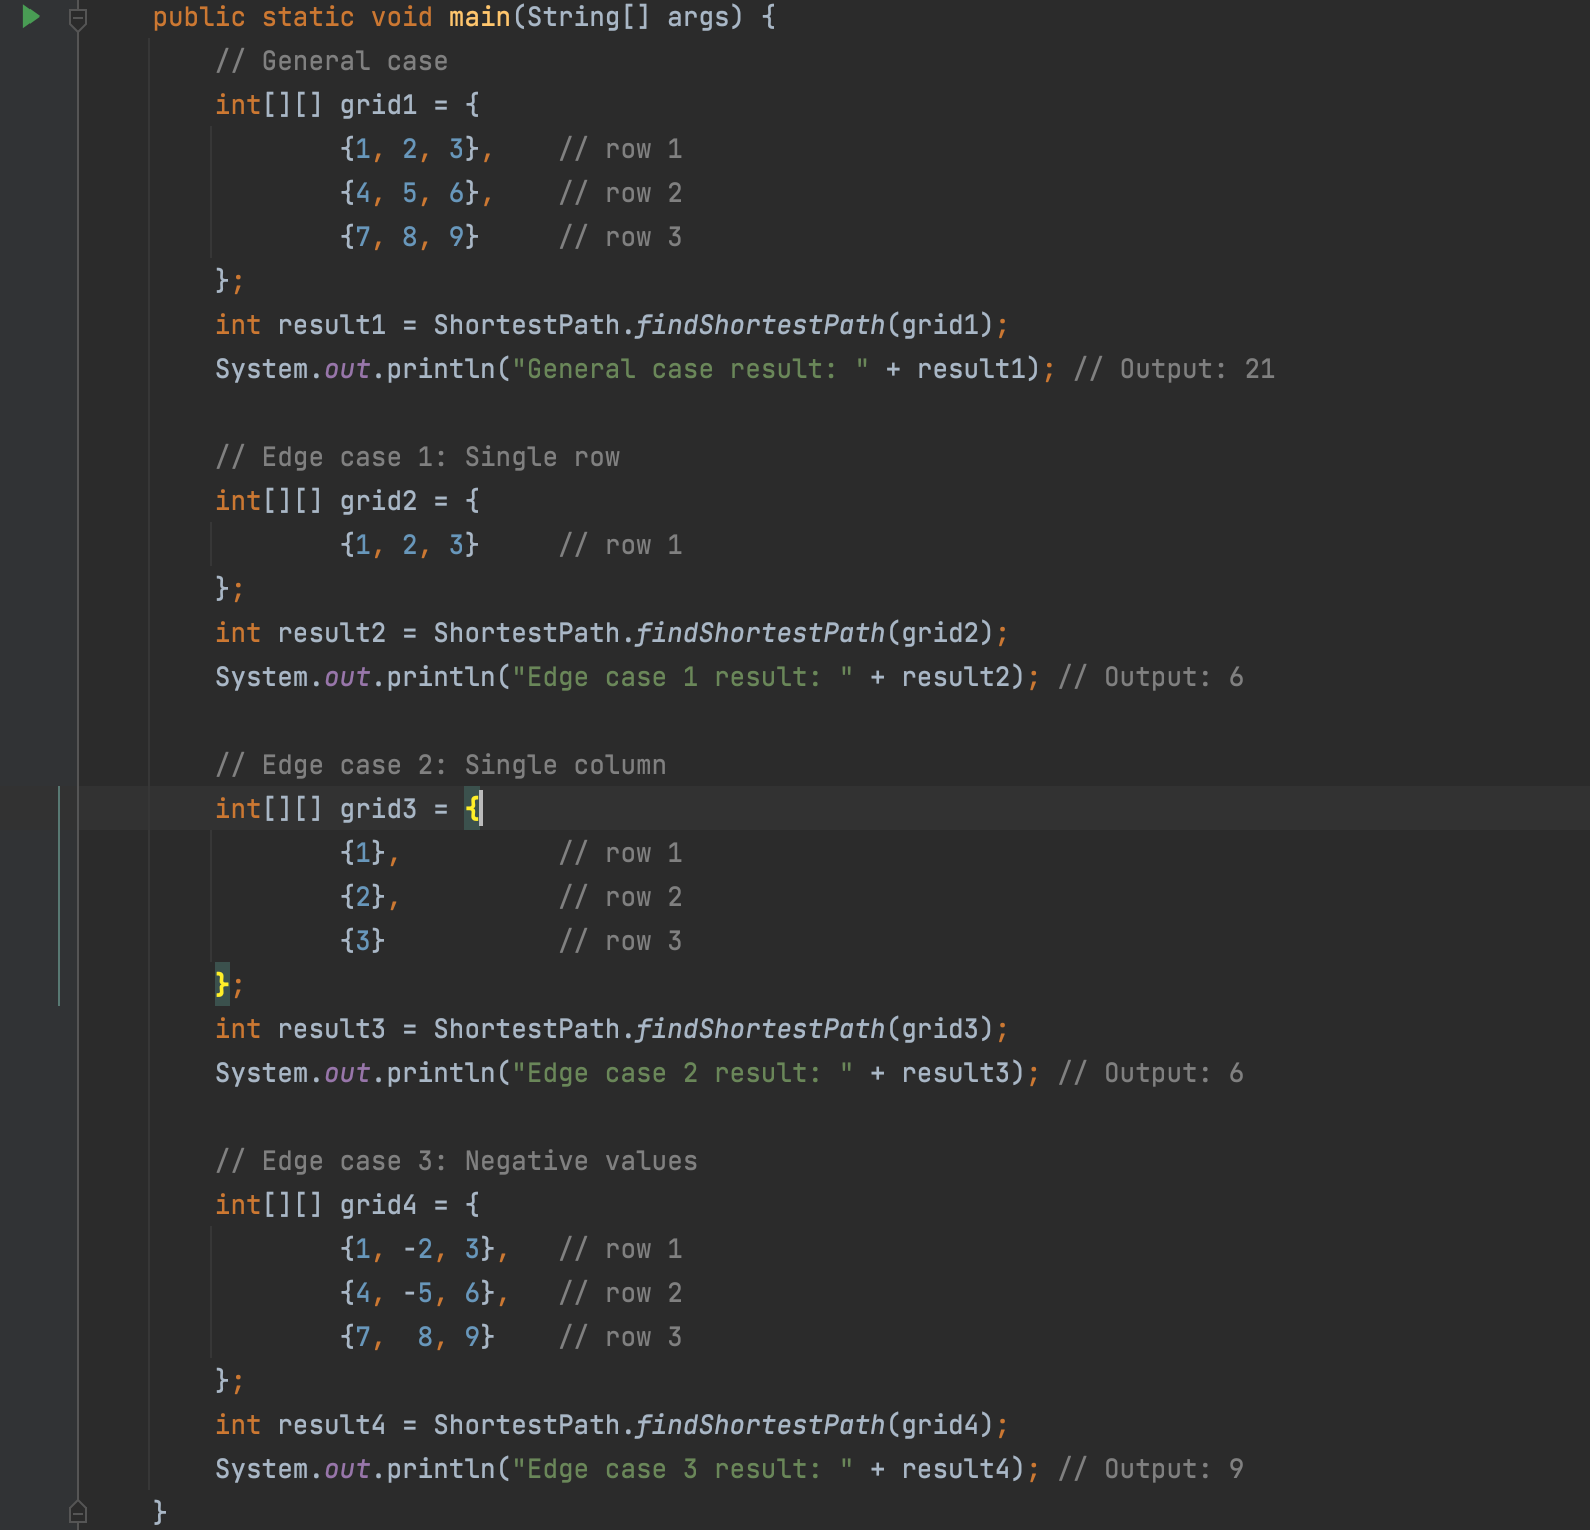
\includegraphics[scale=0.5]{figure8.png}
\caption{Main.java - Test cases and execution of the ShortestPath algorithm}
\end{figure}

\begin{figure}[h]
\centering
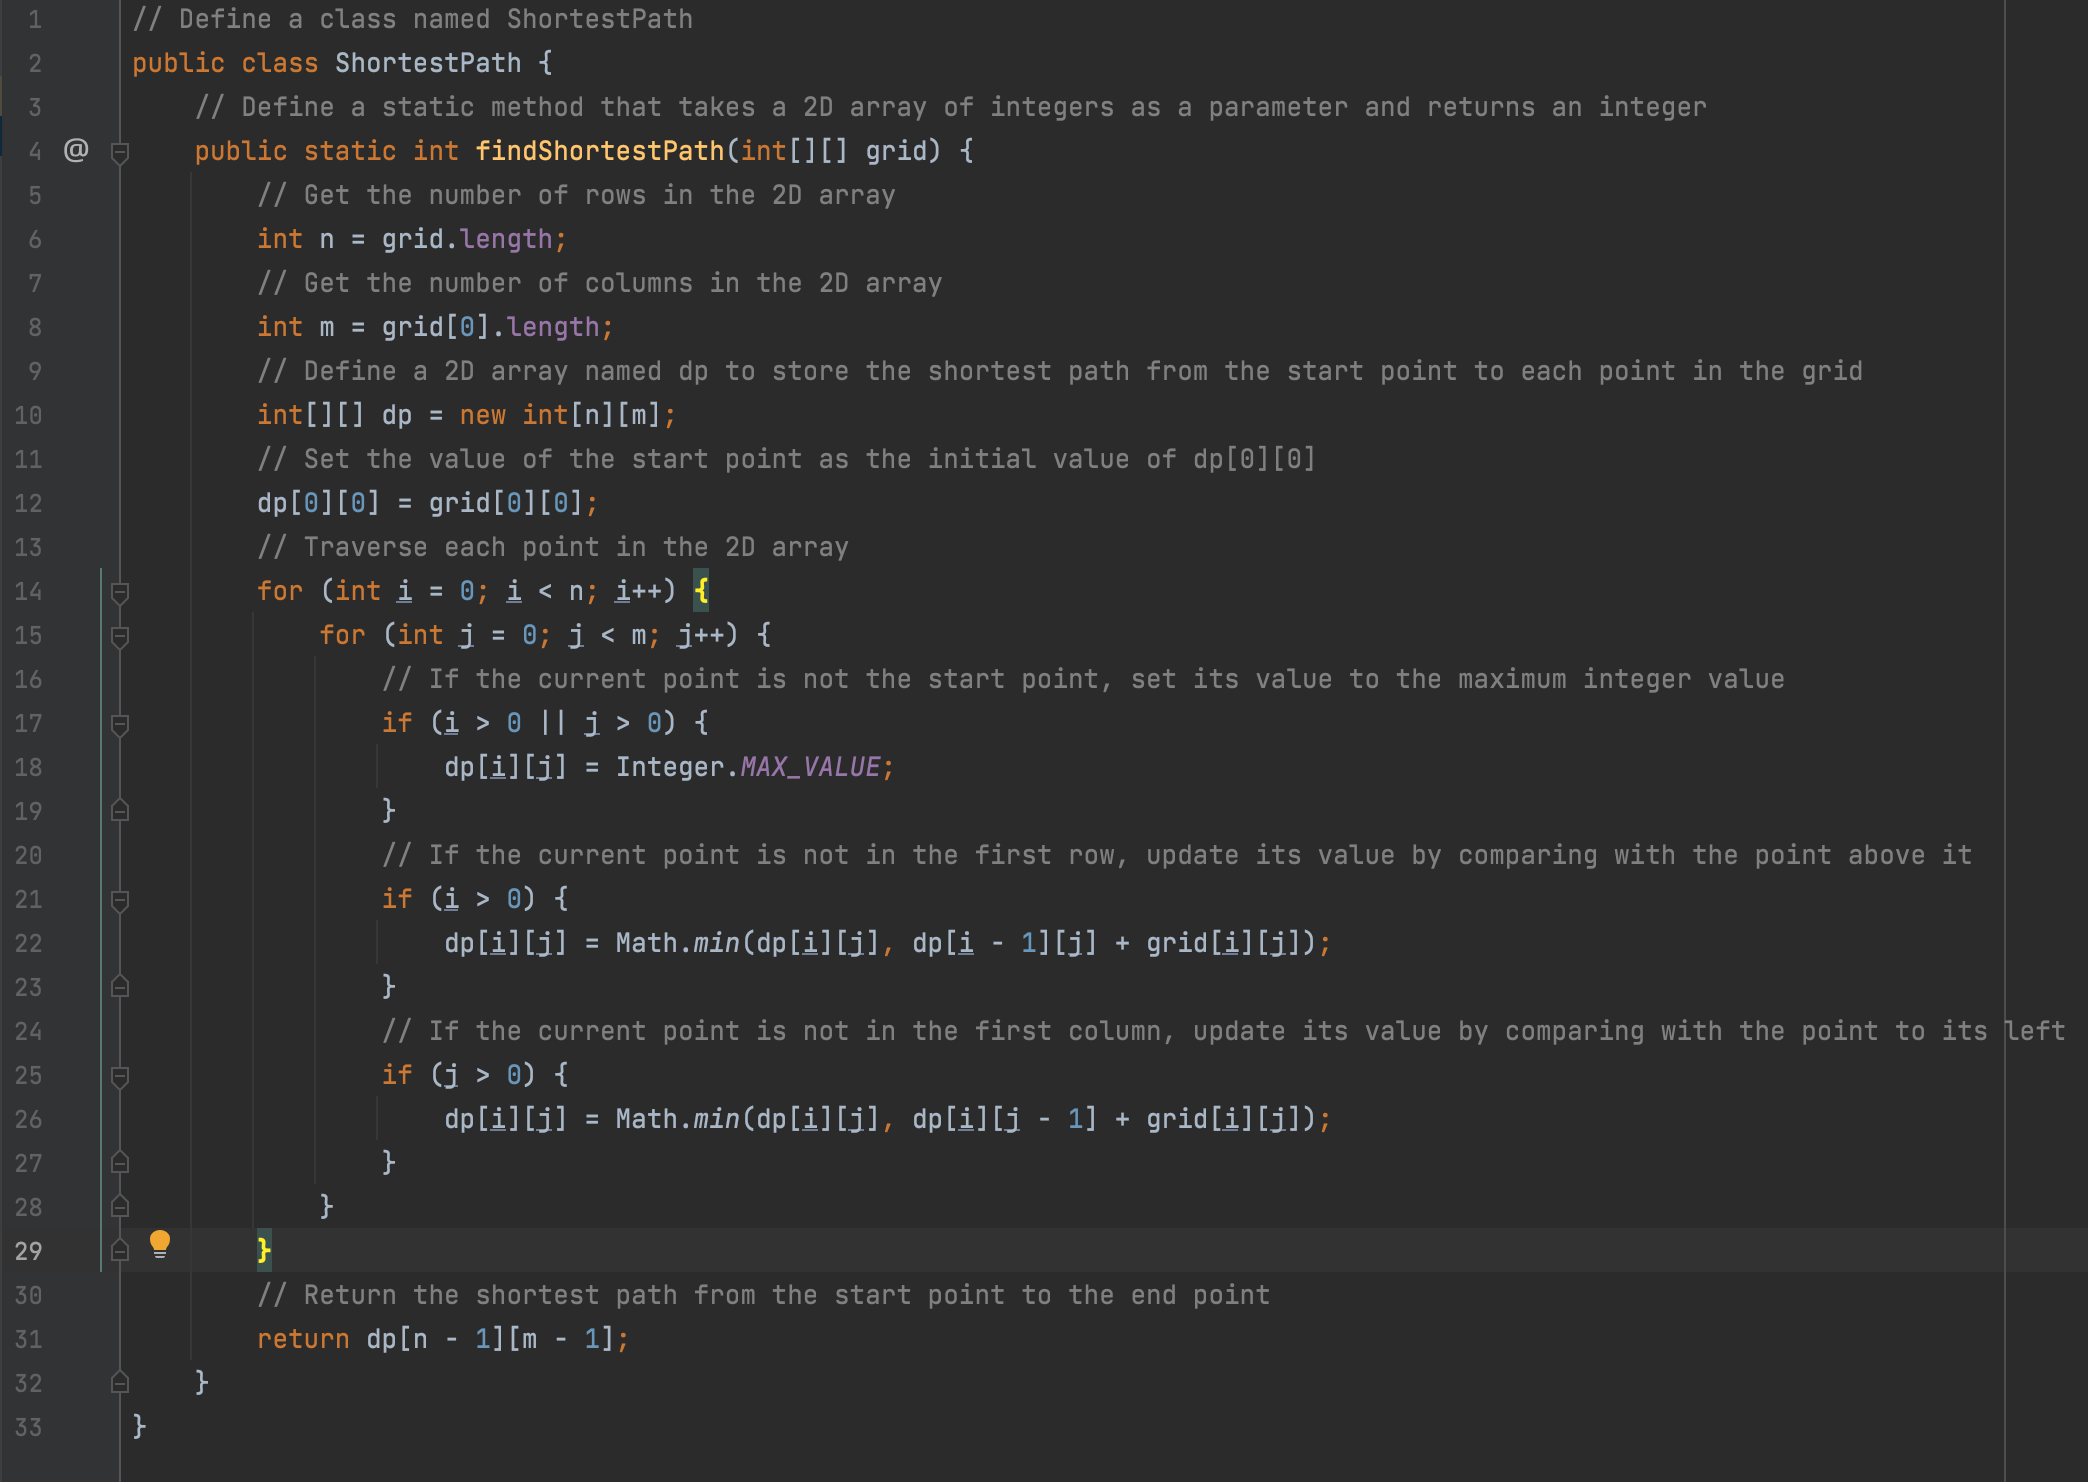
\includegraphics[scale=0.4]{figure9.png}
\caption{ShortestPath.java - Implementation of the dynamic programming algorithm to find the shortest path in a 2D grid}
\end{figure}



\end{document}